\documentclass[aspectratio=169]{beamer}
\usetheme{Singapore}

% add page numbers at the bottom of the slides
\setbeamertemplate{caption}[numbered]
\addtobeamertemplate{navigation symbols}{}{%
    \usebeamerfont{footline}%
    \usebeamercolor[fg]{footline}%
    \hspace{1em}%
    \raisebox{1.4pt}[0pt][0pt]{\insertframenumber/\inserttotalframenumber}
}

% \definecolor{primarycolor}{HTML}{0000FF}

% \makeatletter

% \def\sectioncolor{primarycolor}% color to be applied to section headers

% \setbeamercolor{palette primary}{use=structure,fg=structure.fg}
% \setbeamercolor{palette secondary}{use=structure,fg=structure.fg!75!black}
% \setbeamercolor{palette tertiary}{use=structure,fg=structure.fg!50!black}
% \setbeamercolor{palette quaternary}{fg=black}

% \setbeamercolor{local structure}{fg=primarycolor}
% \setbeamercolor{structure}{fg=primarycolor}
% \setbeamercolor{title}{fg=primarycolor}
% \setbeamercolor{section in head/foot}{fg=black}

% \setbeamercolor{normal text}{fg=black,bg=white}
% \setbeamercolor{block title alerted}{fg=red}
% \setbeamercolor{block title example}{fg=primarycolor}

% \setbeamercolor{footline}{fg=primarycolor!50}
% \setbeamerfont{footline}{series=\bfseries}

% use classic LaTeX font for maths
\usefonttheme[onlymath]{serif}

\usepackage{cmap}
\usepackage[english]{babel}
\usepackage[T1]{fontenc}
\usepackage[utf8]{inputenc}
\usepackage[kerning=true]{microtype}
\usepackage{lmodern}

\usepackage{amsmath}
\usepackage{amsfonts}
\usepackage{amssymb}
\usepackage{amsthm}

\usepackage{mathtools}
\usepackage{booktabs}
\newcommand{\tabitem}{~~\llap{\textbullet}~~}

\usepackage[
    backend=biber,
    style=numeric,
]{biblatex}
\usepackage{graphicx}
\usepackage[justification=centering]{caption}
\usepackage{csquotes}
\usepackage{minted}


\graphicspath{{./images/}}

\addbibresource{../report/report.bib}

\AtBeginSection[]
{
  \begin{frame}
    \frametitle{Plan}
    \tableofcontents[currentsection]
  \end{frame}
}

\title{\textbf{Implementation of an\\Iterative Linear Quadratic Regulator (iLQR)}}
\author{Gabriel Desfrene\and Antoine Groudiev}

\titlegraphic{
\includegraphics[height=1.8cm]{./images/logo-ens-psl.png}}

\date{January 15, 2025}

\begin{document}
\frame{\titlepage}

\begin{frame}{Plan}
    \tableofcontents
\end{frame}

\section{Problem statement}
\begin{frame}{General formulation}
    \begin{itemize}
        \item Dynamics function:
              \begin{equation*}
                  x_{t+1} = f(x_t, u_t)
              \end{equation*}
        \item Goal: minimize a quadratic cost function
        \item Cost function:
              \begin{equation*}
                  J(u) = \sum_{t=0}^{T-1} \left(x_t^\top Q x_t + u_t^\top R u_t\right) + \frac{1}{2}(x_T-x^*)^\top Q_f (x_T-x^*)
              \end{equation*}
        \item $Q$: state cost matrix
        \item $Q_f$: final state cost matrix
        \item $R$: control cost matrix
    \end{itemize}
\end{frame}

\begin{frame}{Example: Simple Pendulum}
    \begin{minipage}[c]{0.6\linewidth}
        \begin{itemize}
            \item State: $x = [\theta\:\:\:\dot{\theta}]$
            \item Control: $u$, torque applied to the pendulum
            \item Dynamics: physical laws (simulator)
            \item Target: $x=[0\:\:\:0]$
            \item Cost function:
                  \begin{equation*}
                      J(u) = \frac{1}{2}\left(\theta_f^2+\dot{\theta}_f^2\right) + \frac{1}{2}\int_0^T ru^2(t) \mathrm{d} t
                  \end{equation*}
                  corresponding to $Q_f = I_2$, $Q=0_2$, $R=rI_1$
        \end{itemize}
    \end{minipage}
    \hspace{0.25cm}
    \begin{minipage}[c]{0.35\linewidth}
        \begin{figure}
            \centering
            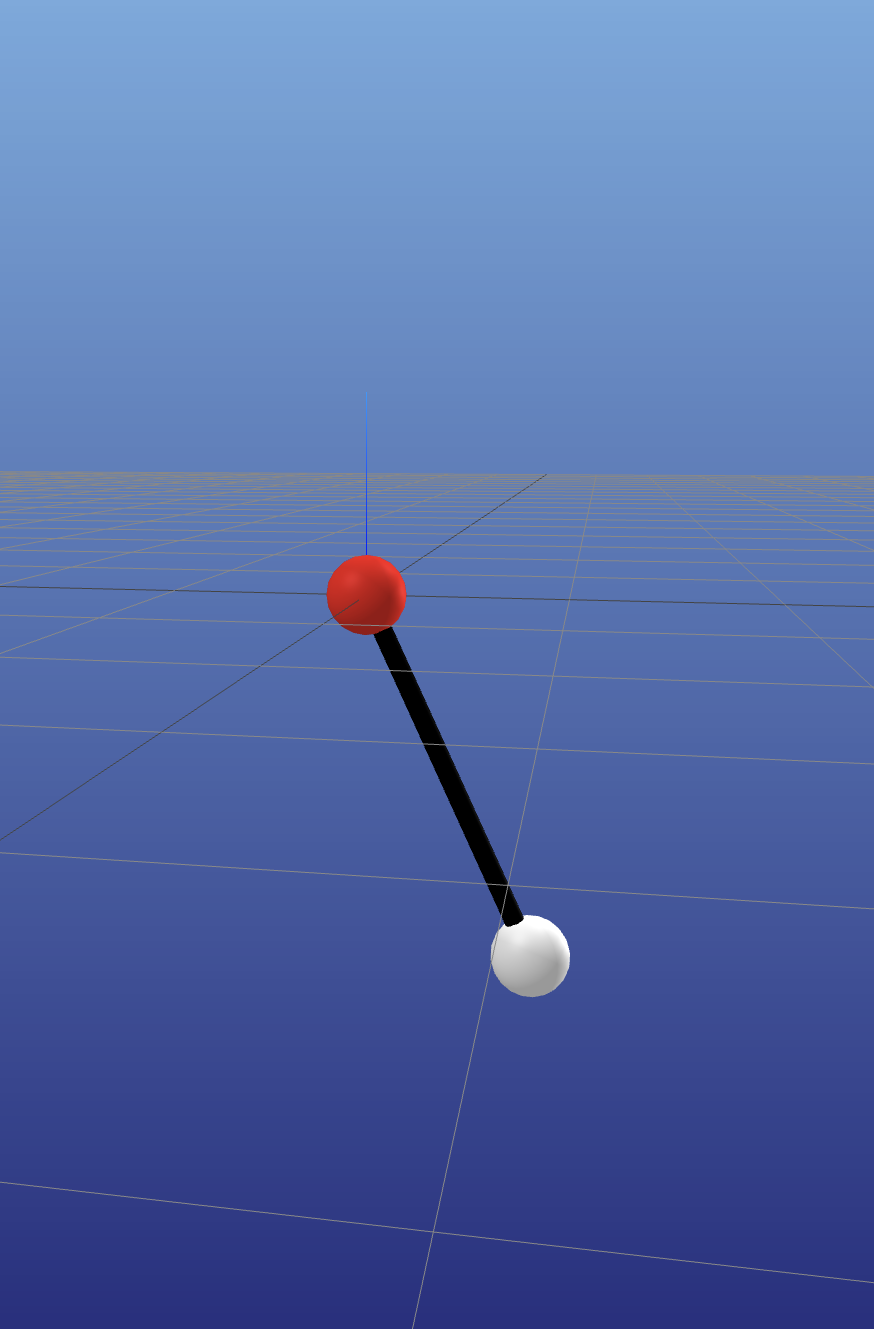
\includegraphics[width=0.7\linewidth]{pendulum.png}
        \end{figure}
    \end{minipage}
\end{frame}

\begin{frame}{Example: Cartpole}
    \begin{minipage}[c]{0.6\linewidth}
        \begin{itemize}
            \item State: $x=[y\:\:\:\theta\:\:\:\dot{y}\:\:\:\dot{\theta}]$
            \item Control: $u$, force applied to the cart
            \item Dynamics: physical laws (simulator)
            \item Target: $x=[0\:\:\:0\:\:\:0\:\:\:0]$
            \item Cost function:
                  \begin{equation*}
                      J(u) = \frac{1}{2}\left(\theta_f^2+\dot{\theta}_f^2 + y_f^2 + \dot{y}_f^2\right) + \frac{1}{2}\int_0^T ru^2(t) \mathrm{d} t
                  \end{equation*}
                  corresponding to $Q_f = I_4$, $Q=0_4$, $R=rI_1$
        \end{itemize}
    \end{minipage}
    \hspace{0.25cm}
    \begin{minipage}[c]{0.35\linewidth}
        \begin{figure}
            \centering
            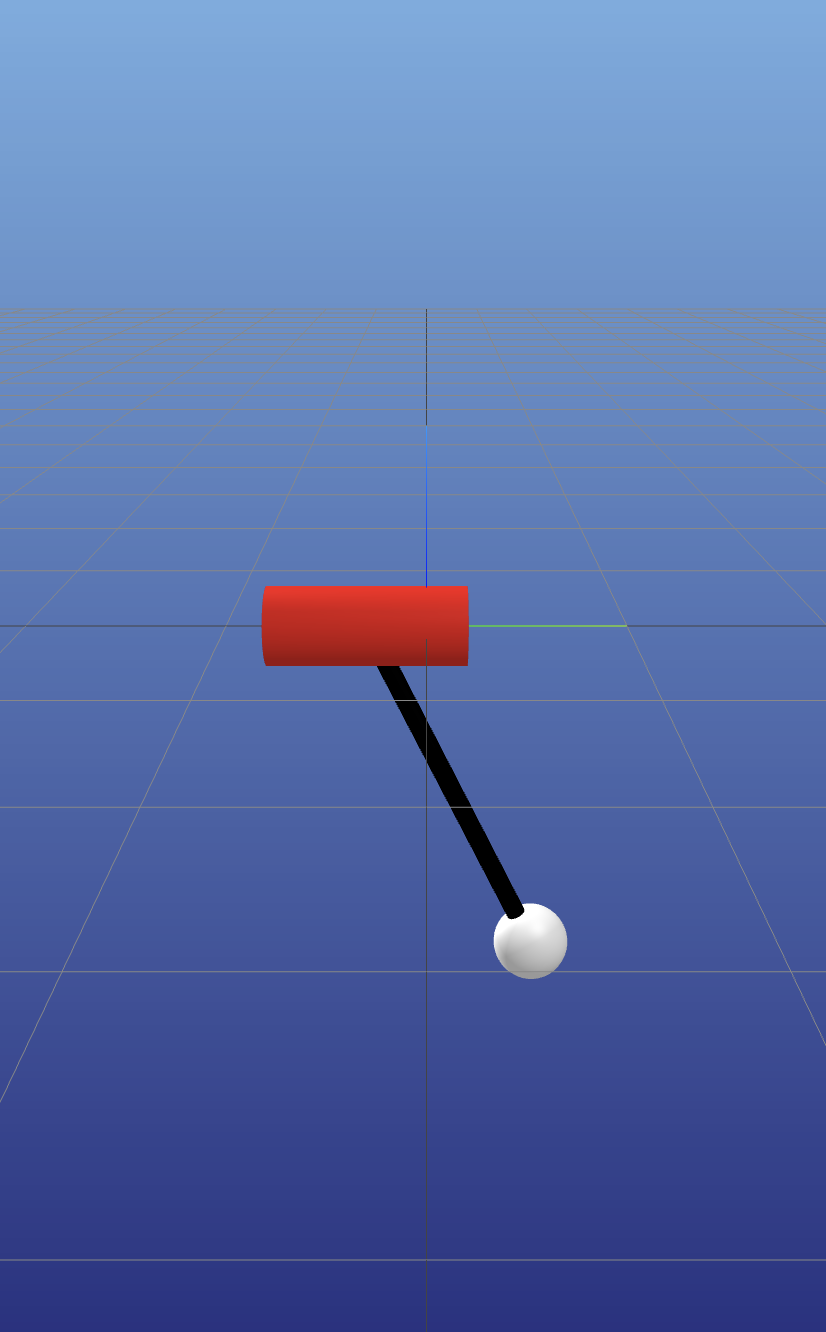
\includegraphics[width=0.7\linewidth]{cartpole.png}
        \end{figure}
    \end{minipage}
\end{frame}

\section{The iLQR algorithm}
\begin{frame}{General idea}
    \begin{itemize}
        \item iLQR is an iterative algorithm
        \item Start with an initial trajectory
        \item Iteratively improve it using a local linear approximation
        \item Stop when the trajectory converges
    \end{itemize}
\end{frame}

\begin{frame}{Linearizing the dynamics}
    The equation $x_{t+1} = f(x_t, u_t)$ is linearized (at each step) as:
    \begin{equation*}
        \delta x_{t+1} = A_t \delta x_t + B_t \delta u_t
    \end{equation*}
    with:
    \begin{itemize}
        \item $A_t$: Jacobian of $f$ with respect to $x$ evaluated at $(x_t, u_t)$
        \item $B_t$: Jacobian of $f$ with respect to $u$ evaluated at $(x_t, u_t)$
    \end{itemize}
    We are in LQR (Linear Quadratic Regulator, cf. TP5) setup!
\end{frame}

\begin{frame}{Trajectory refinement using LQR}
    \begin{enumerate}
        \item \textbf{Forward pass}: compute the successive states $(x_t)$ for the current controls $(u_t)$, and the corresponding cost $J$
        \item \textbf{Backward pass}: compute the gains, i.e. how much we should change the controls in each direction to minimize the cost
        \item \textbf{Forward rollout}: apply the gains to the controls to obtain a new trajectory
        \item Repeat until convergence
    \end{enumerate}
    \vspace*{1cm}
    For the complete derivations, see \cite{jackson2019ilqr} or \cite{harley2020ilqr}.
\end{frame}

\begin{frame}{Computing the Jacobians}{Finite differences method}
    We want to compute:
    \begin{itemize}
        \item $A_t=\frac{\partial f}{\partial x}(x_t, u_t)$, i.e. how much the state at time $t+1$ changes when we slightly change the state at time $t$
        \item $B_t=\frac{\partial f}{\partial u}(x_t, u_t)$, i.e. how much the state at time $t+1$ changes when we slightly change the control at time $t$
    \end{itemize}
    In a black box setting, we can use finite differences:
    \begin{align*}
        [A_t]_i & \approx \frac{f(x_t+\varepsilon e_i, u_t)-f(x_t-\varepsilon e_i, u_t)}{2\varepsilon} \\
        [B_t]_i & \approx \frac{f(x_t, u_t+\varepsilon e_i)-f(x_t, u_t-\varepsilon e_i)}{2\varepsilon}
    \end{align*}
    for some small $\varepsilon$ and the canonical basis $(e_i)$
\end{frame}

\begin{frame}[fragile]{Computing the Jacobians}{Using Pinocchio}
    \begin{minted}{python}
# Jacobians of the Articulated-Body algorithm
J1_q, J1_v, J1_u = pin.computeABADerivatives(model, data_sim, q, v, u)

# compute the Jacobians of the integration on SE(...)
J2_q, J2_v_2 = pin.dIntegrate(model, q, v_2 * dt)
    \end{minted}
\end{frame}

\begin{frame}{Tricks for practical convergence}
    \begin{itemize}
        \item \textbf{Gradient clipping}: limit the size of the control updates norm to $\alpha$ to avoid divergence
              \begin{equation*}
                  \delta u_t = \frac{\delta u_i}{\max\left(1, \frac{\|\delta u_i\|}{\alpha}\right)}
              \end{equation*}
        \item \textbf{Gaussian initialization}: start with a small random control sequence instead of a zero sequence
              \begin{equation*}
                  u_t \sim \mathcal{N}(0, \Sigma)
              \end{equation*}
        \item \textbf{Regularization based on Levenberg-Marquardt}: When inverting the $Q_{uu}$ matrix, add a dynamic regularization term $\mu > 0$ to ensure positive definiteness
              \begin{equation*}
                  Q_{uu} = U\Sigma U^{\mathrm{T}} \rightarrow Q_{uu}^{-1} = U\Sigma' U^{\mathrm{T}}
                  \quad\text{with}\quad
                  \Sigma' = \begin{cases}
                      0                         & \text{if $\sigma_i\leqslant 0$} \\
                      \dfrac{1}{\sigma_i + \mu} & \text{otherwize}
                  \end{cases}
              \end{equation*}
    \end{itemize}
\end{frame}

\section{Our implementation}
\begin{frame}{What language to use?}
    \begin{figure}
        \centering
        \renewcommand{\arraystretch}{1.4}
        \begin{tabular}{p{5cm}p{3.5cm}p{4.5cm}}
            \centering\textbf{Python}           & \centering\textbf{C++}  & \hspace{1.6cm}\textbf{Rust}       \\
            \tabitem Easy to use                & \tabitem "Fast"           & \tabitem "Fast"                     \\
            \tabitem Support for many libraries & \tabitem Not very funny & \tabitem Easy bindings for Python \\
            \tabitem Embarrassingly slow        &                         & \tabitem Very funny
        \end{tabular}
    \end{figure}
    \vspace*{1cm}
    \centering
    Therefore, we chose to have a Rust core with Python bindings
    % \begin{minipage}[c]{0.3\linewidth}
    %     \textbf{Python}
    %     \begin{itemize}
    %         \item Easy to use
    %         \item Bindings for many libraries
    %         \item Embarrassingly slow
    %     \end{itemize}
    % \end{minipage}
    % \hspace{0.25cm}
    % \begin{minipage}[c]{0.3\linewidth}
    %     \textbf{C++}
    %     \begin{itemize}
    %         \item Fast
    %         \item Not very funny
    %     \end{itemize}
    % \end{minipage}
    % \hspace{0.25cm}
    % \begin{minipage}[c]{0.3\linewidth}
    %     \textbf{Rust}
    % \end{minipage}
\end{frame}

\begin{frame}{From Rust to Python, and the other way around}
    \begin{itemize}
        \item Instantiate the solver in Python
        \item Use Python libraries to define the dynamics
        \item The Rust solver does the computations, and calls the Python \texttt{dynamics} function and the Pinocchio functions for the Jacobians
        \item Supports both methods for computing the Jacobians
    \end{itemize}
\end{frame}

\begin{frame}[fragile]{API Basic usage}
    \begin{minted}{python}
def dynamics(x, u):
    return ... # simulator

Q = np.zeros((state_dim, state_dim)) # state cost
Qf = np.eye(state_dim) # final state cost
R = 1e-5 * np.eye(control_dim) # control cost (minimize the energy)

s = ilqr.ILQRSolver(state_dim, control_dim, Q, Qf, R)
target = np.zeros(state_dim) # upright pendulum with no velocity
output = s.solve(np.concatenate((q0, v0)), target, dynamics, time_steps=N,
                 gradient_clip=10.0,  # max norm of the gradient
                 initialization=0.5)  # std of the Gaussian initialization
\end{minted}
\end{frame}

\section{Demonstration time}
\begin{frame}
    \begin{center}
        \huge Demonstration time!
    \end{center}
\end{frame}

\begin{frame}{References}
    \nocite{*}
    \printbibliography{}
\end{frame}

\end{document}
